\subsection{ROLAP Schema}
    \subsubsection{Description}
        Views are just joins between fact and dimension tables, replacing ids with their textual representations, proving better readability.

    \subsubsection{Dimensions}
        \begin{itemize}
    \item Category
    
    \item Country
    \begin{itemize}
        \item Different granularity in the same column
        \item Use queries such as \code{WHERE country LIKE `Italy\%'}
        \item Example:
        \begin{itemize}
            \item \textit{Italy}
            \item \textit{Italy\_NORD}
            \item \textit{Italy\_CNOR}
            \item \textit{Italy\_CSUD}
            \item \textit{Italy\_SUD}
            \item \textit{Italy\_SICI}
            \item \textit{Italy\_SARD}
            \item ...
        \end{itemize}
    \end{itemize}
    
    \item Energy source
    
    \item Future product
    \begin{itemize}
        \item 2-level aggregation (future days, weeks)
        \begin{itemize}
            \item Offset (D+n / W+n / M+n / ...)
            \item Offset type
            \begin{itemize}
                \item Day 
                \item Weekend 
                \item Week 
                \item Month 
                \item Quartet 
                \item Year 
                \item BOM
            \end{itemize}
        \end{itemize}
    \end{itemize}
    
    \item Granularity
    
    \item Holiday
    \begin{itemize}
        \item Start
        \item Holiday name
        \item Country (dimension)
    \end{itemize}
    
    \item Model
    
    \item Outage status
    
    \item Outage type
    
    \item Power plant
    \begin{itemize}
        \item Power Plant (same plant, multiple codes; mostly 1-1)
        \item Code (same code, multiple plants; mostly 1-1)
        \item Energy source (dimension)
        \item Technology (dimension)
        \item Country (dimension)
        \item Capacity
        \item Plant type
        \item Plant father (dimension, self)
    \end{itemize}
    
    \item Profile
    
    \item Provider
    
    \item Scenario
    
    \item Technology
    
    \item Unit
    
    \item Version
\end{itemize} 
        
    \subsubsection{Facts}
        \begin{itemize}
    \item Aggregated curve
    
    \item CBCO
    \begin{itemize}
        \item Limiti capacita` linee elettriche europee
        \begin{itemize}
            \item Si usano per ricavare i prezzi di trasporto energia
        \end{itemize}
        
        \item Contiene tutti i vincoli possibili, non solo quelli limitanti
    \end{itemize}
    
    \item Flow (FCT/RLZ)
    \begin{itemize}
        \item Trasmissione di energia tra countries
    \end{itemize}
    
    \item Job
    \begin{itemize}
        \item Tutti i FCT hanno un publication time
        \begin{itemize}
            \item Per evitare di importare due volte gli stessi dati
        \end{itemize}
    \end{itemize}
    
    \item PDTF
    \begin{itemize}
        \item Vincoli limitanti su capacita` linee elettriche europee
        \item Sono scaricati, ma si potrebbero anche ricavare da CBCO (WIP)
        \item Contiene l'1.74\% dei dati di CBCO
    \end{itemize}
    
    \item Timeseries (FCT/RLZ)
    \begin{itemize}
        \item Consumi
    \end{itemize}
    
    \item Unavailability
    \begin{itemize}
        \item Outages on power plants
    \end{itemize}
    
    \item Volatility/Correlation
    \begin{itemize}
        \item Model coefficients, computed from prices
    \end{itemize}
    
\end{itemize}
        
    \begin{figure}
        \centering
        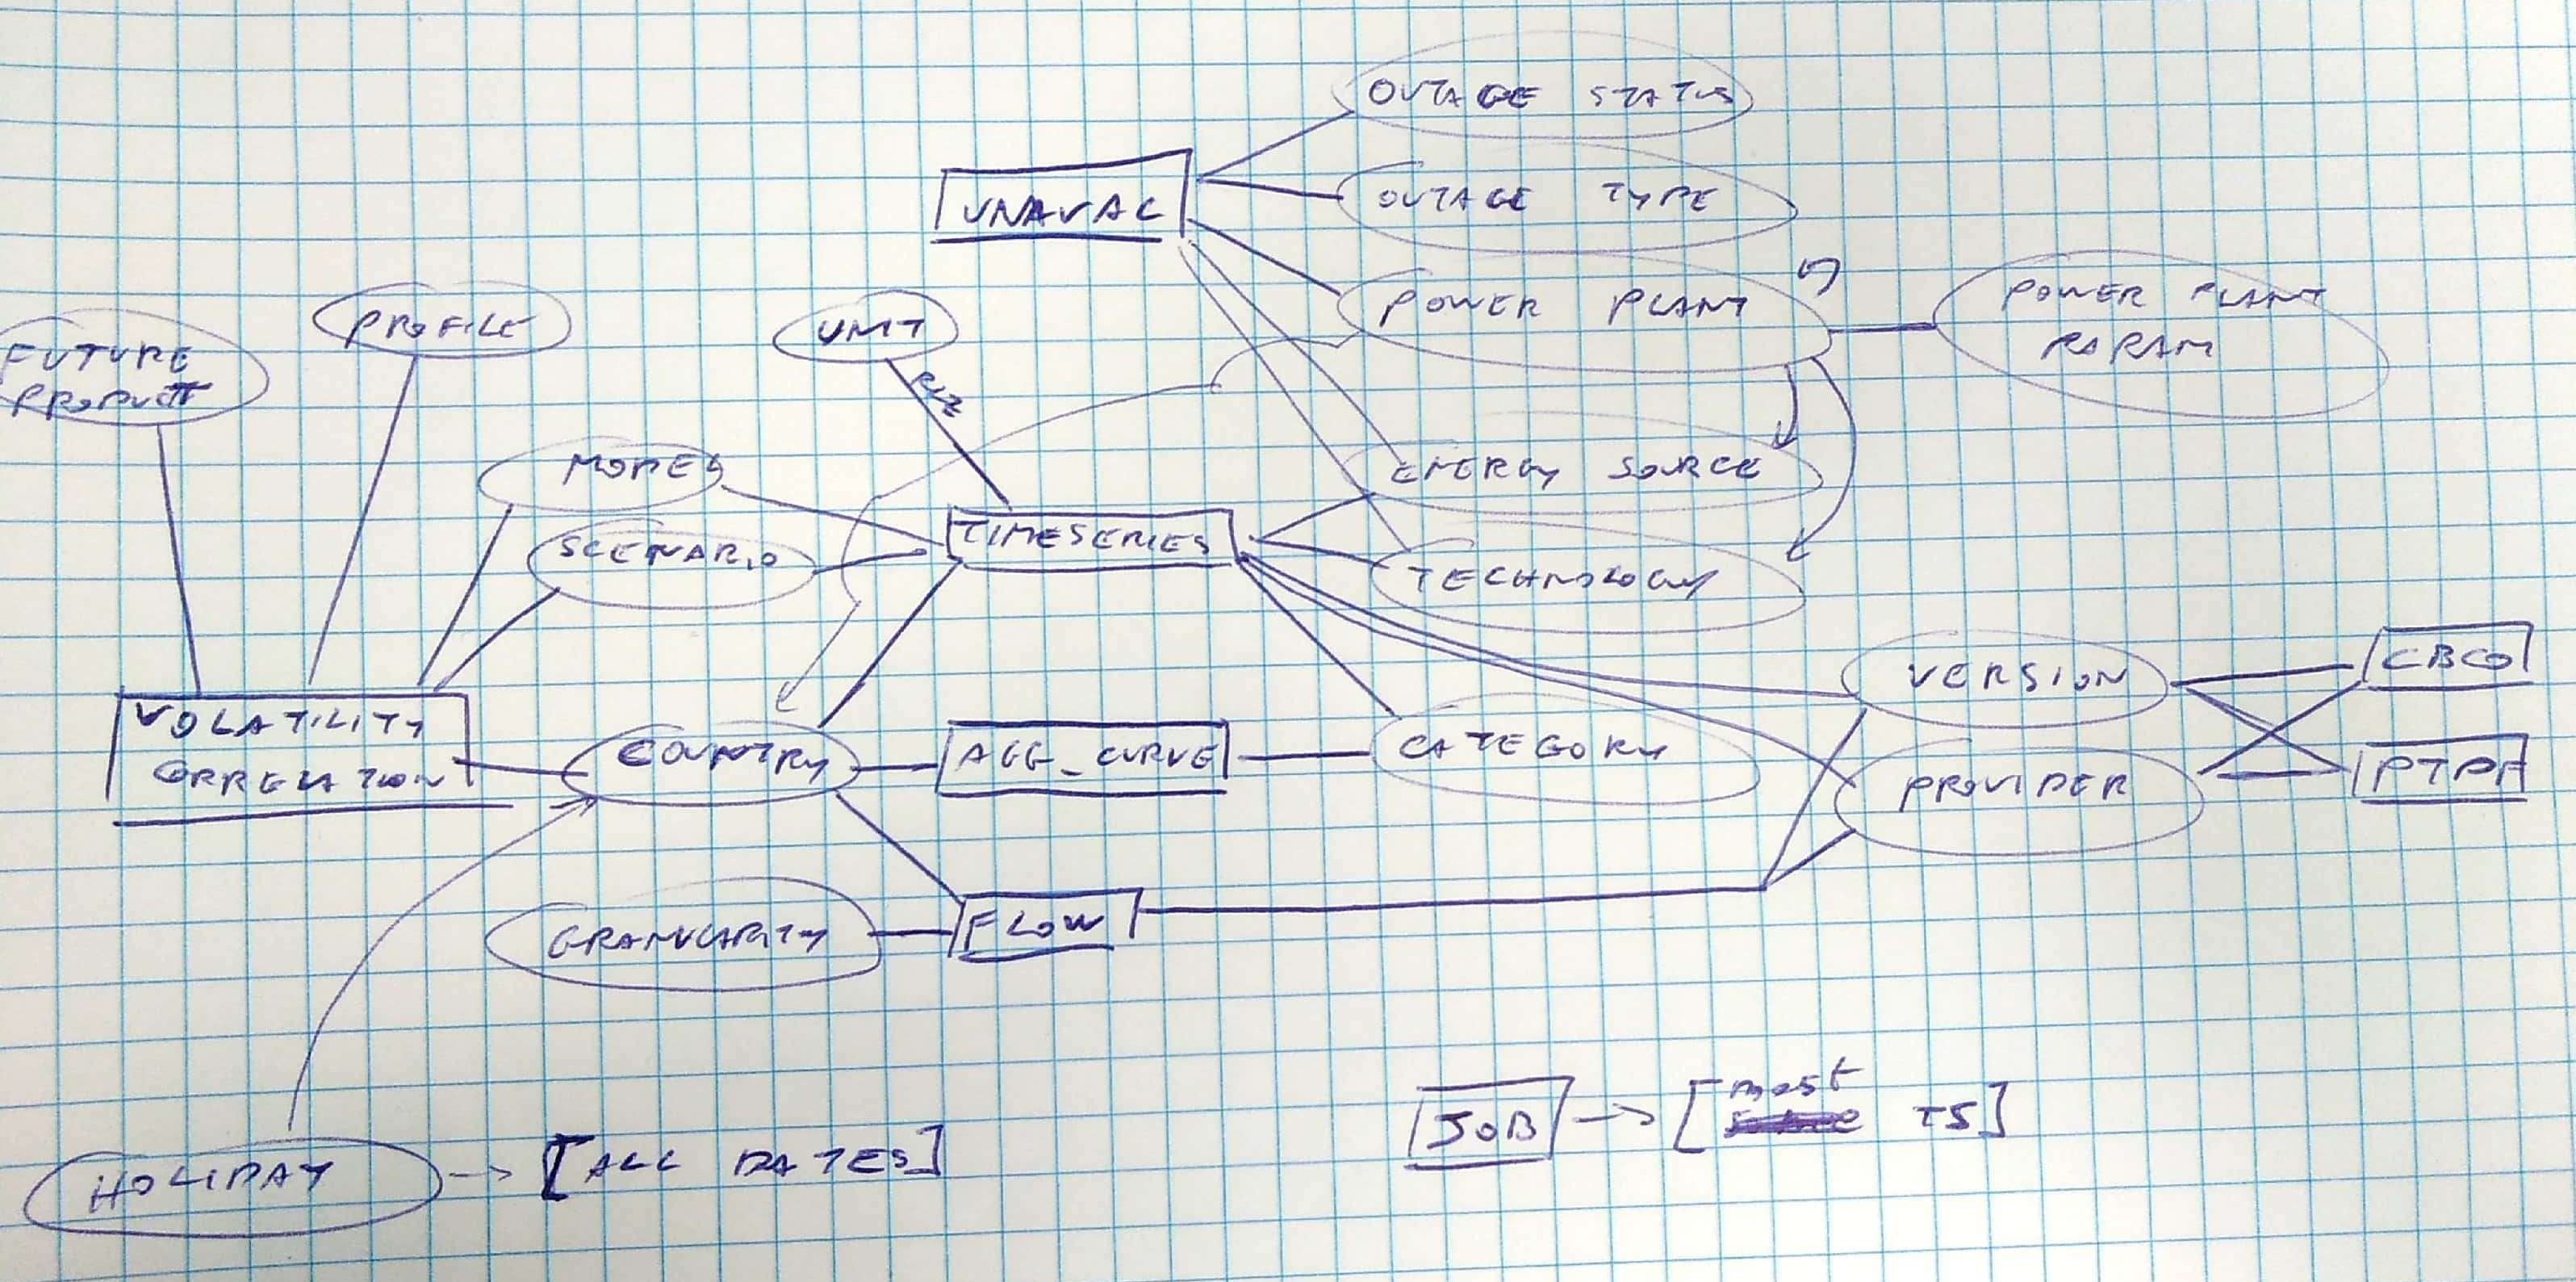
\includegraphics[width=\textwidth]{res/img/schema_db.jpg}
        \caption{DB Schema. Circles represent dimensions; rectangles facts.}
        \label{fig:db_schema}
    \end{figure}
    
\subsection{Usage}
    A \textit{Julia} script is run every 30 minutes with some default parameters.
    Additionally, it can be manually launched from an Excel spreadsheet with custom-set parameters.
    
    \paragraph{Output} In case of a scheduled jobs the results are saved to the db, otherwise they are shown on the spreadsheet.
    
    \paragraph{Goal} The goal is to predict market prices for the following day, on different markets.
    
    \subsubsection{Workflow}
    The script executes the following actions:
    \begin{enumerate}
        \item Data acquisition
        \begin{itemize}
            \item Curves
            \item Realized flows
            \item PTDF
            \item Capacities
            \item Block bids
            \item Consumption FCT timeseries
        \end{itemize}
        
        \item Consumption computations with ML
        
        \item Market model
        \begin{itemize}
            \item Requires all data previously produced
            \item Produces market prices for the following day
        \end{itemize}
    \end{enumerate}
    
    The results are either saved to db or shown to the user.
    
    At 12.42 the stock market shows the official prices, which are used as input for the following day.